\documentclass[11pt,a4paper]{report}
\usepackage[textwidth=37em,vmargin=30mm]{geometry}
\usepackage{calc,xunicode,amsmath,amssymb,paralist,enumitem,tabu,booktabs,datetime2,xeCJK,xeCJKfntef,listings}
\usepackage{tocloft,fancyhdr,tcolorbox,xcolor,graphicx,eso-pic,xltxtra,xelatexemoji}

\newcommand{\envyear}[0]{2025}
\newcommand{\envdatestr}[0]{2025-09-05}
\newcommand{\envfinaldir}[0]{webdb/2025/20250905/final}

\usepackage[hidelinks]{hyperref}
\hypersetup{
    colorlinks=false,
    pdfpagemode=FullScreen,
    pdftitle={Web Digest - \envdatestr}
}

\setlength{\cftbeforechapskip}{10pt}
\renewcommand{\cftchapfont}{\rmfamily\bfseries\large\raggedright}
\setlength{\cftbeforesecskip}{2pt}
\renewcommand{\cftsecfont}{\sffamily\small\raggedright}

\setdefaultleftmargin{2em}{2em}{1em}{1em}{1em}{1em}

\usepackage{xeCJK,xeCJKfntef}
\xeCJKsetup{PunctStyle=plain,RubberPunctSkip=false,CJKglue=\strut\hskip 0pt plus 0.1em minus 0.05em,CJKecglue=\strut\hskip 0.22em plus 0.2em}
\XeTeXlinebreaklocale "zh"
\XeTeXlinebreakskip = 0pt


\setmainfont{Brygada 1918}
\setromanfont{Brygada 1918}
\setsansfont{IBM Plex Sans}
\setmonofont{JetBrains Mono NL}
\setCJKmainfont{Noto Serif CJK SC}
\setCJKromanfont{Noto Serif CJK SC}
\setCJKsansfont{Noto Sans CJK SC}
\setCJKmonofont{Noto Sans CJK SC}

\setlength{\parindent}{0pt}
\setlength{\parskip}{8pt}
\linespread{1.15}

\lstset{
	basicstyle=\ttfamily\footnotesize,
	numbersep=5pt,
	backgroundcolor=\color{black!5},
	showspaces=false,
	showstringspaces=false,
	showtabs=false,
	tabsize=2,
	captionpos=b,
	breaklines=true,
	breakatwhitespace=true,
	breakautoindent=true,
	linewidth=\textwidth
}






\newcommand{\coverpic}[2]{
    % argv: itemurl, authorname
    Cover photo by #2~~(\href{#1}{#1})
}
\newcommand{\makeheader}[0]{
    \begin{titlepage}
        % \newgeometry{hmargin=15mm,tmargin=21mm,bmargin=12mm}
        \begin{center}
            
            \rmfamily\scshape
            \fontspec{BaskervilleF}
            \fontspec{Old Standard}
            \fontsize{59pt}{70pt}\selectfont
            WEB\hfill DIGEST
            
            \vfill
            % \vskip 30pt
            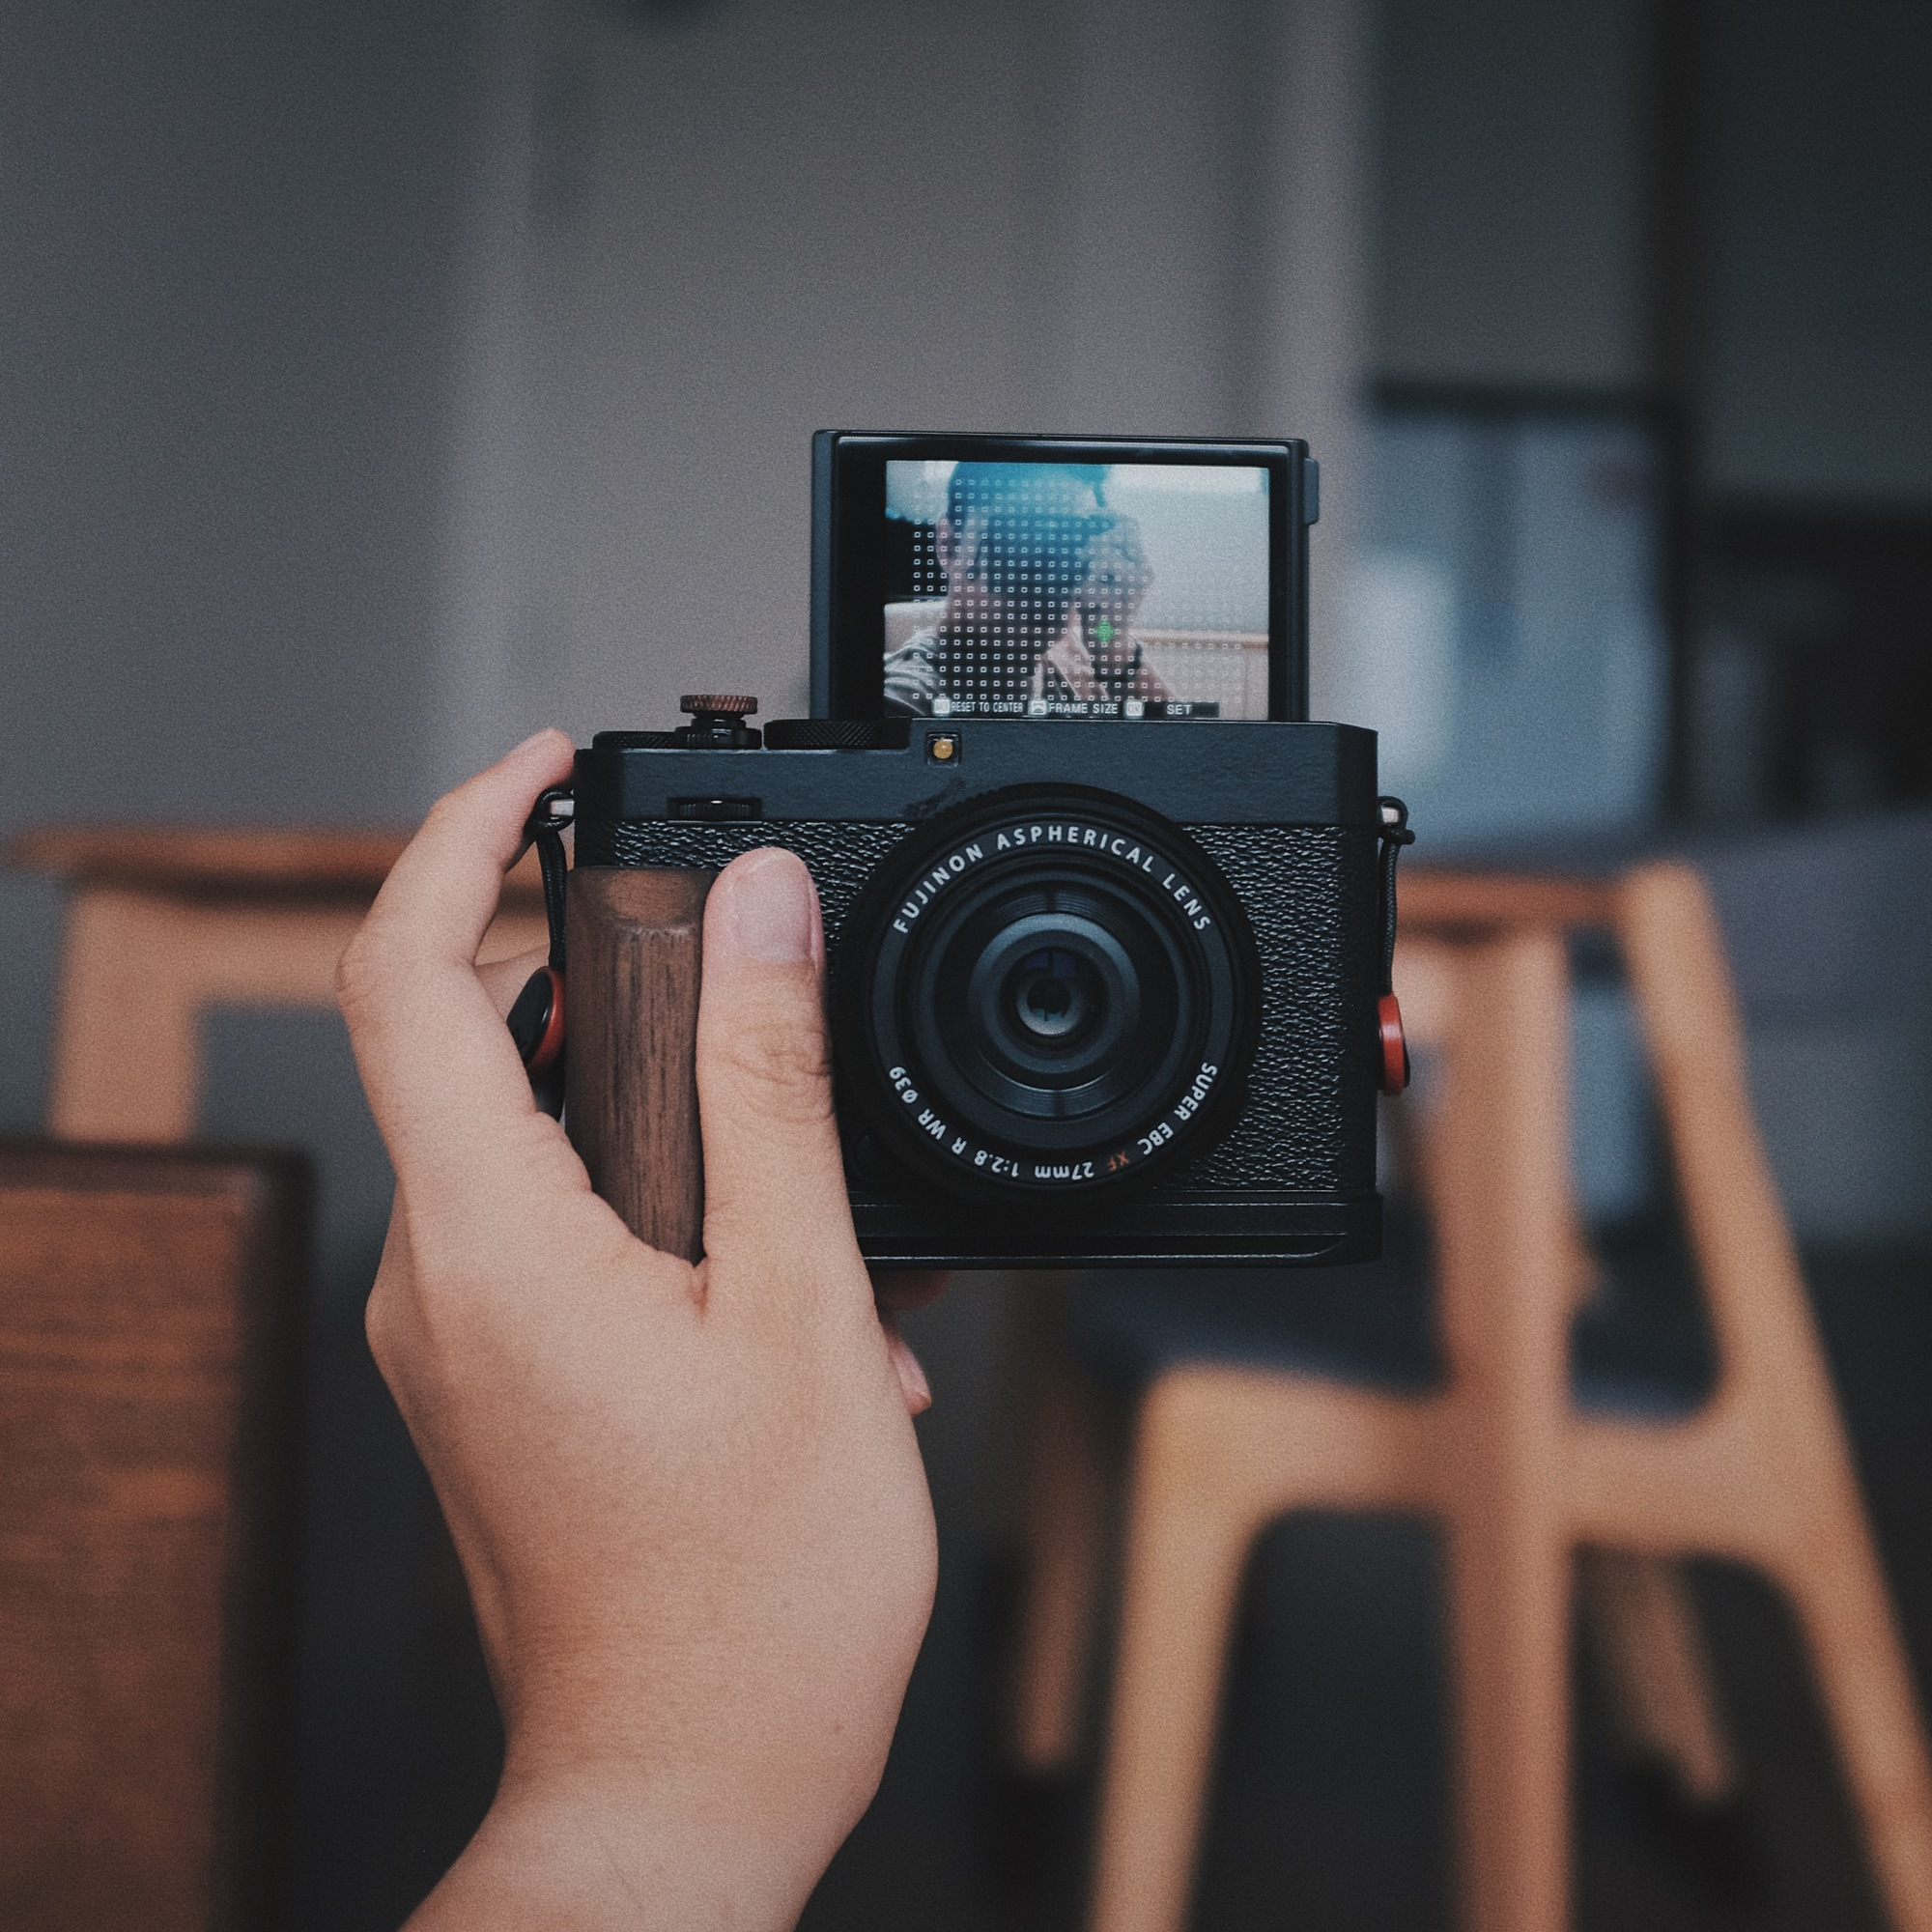
\includegraphics[width=\linewidth]{\envfinaldir/coverpic-prod.jpg}\par
            % \vskip 30pt
            \vfill

            \normalsize\rmfamily\scshape
            \copyright{} The Web Digest Project \hfill\large \envdatestr
        \end{center}
    \end{titlepage}
    % \restoregeometry
}
\newcommand{\simplehref}[1]{%
    \textcolor{blue!80!green}{\href{#1}{#1}}%
}
\renewcommand{\contentsname}{\center\Huge\sffamily\bfseries Contents\par\vskip 20pt}
\newcounter{ipartcounter}
\setcounter{ipartcounter}{0}
\newcommand{\ipart}[1]{
    % \vskip 20pt
    \clearpage
    \stepcounter{ipartcounter}
    \phantomsection
    \addcontentsline{toc}{chapter}{#1}
    % \begin{center}
    %     \Huge
    %     \sffamily\bfseries
    %     #1
    % \end{center}
    % \vskip 20pt plus 7pt
}
\newcounter{ichaptercounter}
\setcounter{ichaptercounter}{0}
\newcommand{\ichapter}[1]{
    % \vskip 20pt
    \clearpage
    \stepcounter{ichaptercounter}
    \phantomsection
    \addcontentsline{toc}{section}{\numberline{\arabic{ichaptercounter}}#1}
    \begin{center}
        \Huge
        \sffamily\bfseries
        #1
    \end{center}
    \vskip 20pt plus 7pt
}
\newcommand{\entrytitlefont}[1]{\subsection*{\raggedright\Large\sffamily\bfseries#1}}
\newcommand{\entryitemGeneric}[2]{
    % argv: title, url
    \parbox{\linewidth}{
        \entrytitlefont{#1}\par\vskip 5pt
        \footnotesize\ttfamily\mdseries
        \simplehref{#2}
    }\vskip 11pt plus 11pt minus 1pt
}
\newcommand{\entryitemGithub}[3]{
    % argv: title, url, desc
    \parbox{\linewidth}{
        \entrytitlefont{#1}\par\vskip 5pt
        \footnotesize\ttfamily\mdseries
        \simplehref{#2}\par\vskip 5pt
        \small\rmfamily\mdseries#3
    }\vskip 11pt plus 11pt minus 1pt
}
\newcommand{\entryitemAp}[3]{
    % argv: title, url, desc
    \parbox{\linewidth}{
        \entrytitlefont{#1}\par\vskip 5pt
        \footnotesize\ttfamily\mdseries
        \simplehref{#2}\par\vskip 5pt
        \small\rmfamily\mdseries#3
    }\vskip 11pt plus 11pt minus 1pt
}
\newcommand{\entryitemHackernews}[3]{
    % argv: title, hnurl, rawurl
    % \parbox{\linewidth}{
    %     \entrytitlefont{#1}\par\vskip 5pt
    %     \footnotesize\ttfamily\mdseries
    %     \simplehref{#3}\par
    %     \textcolor{black!50}{\href{#2}{#2}}
    % }\vskip 11pt plus 11pt minus 1pt
    \begin{minipage}{\linewidth}
            \entrytitlefont{#1}\par\vskip 5pt
            \footnotesize\ttfamily\mdseries
            \simplehref{#3}\par
            \textcolor{black!50}{\href{#2}{#2}}
    \end{minipage}\par\vskip 11pt plus 11pt minus 1pt
}







\begin{document}

\makeheader

\tableofcontents\clearpage




\ipart{Developers}
\ichapter{Hacker News}
\entryitemTwoLinks{LLM Visualization}{https://news.ycombinator.com/item?id=45130260}{https://bbycroft.net/llm}

\entryitemTwoLinks{Age Simulation Suit}{https://news.ycombinator.com/item?id=45129190}{https://www.age-simulation-suit.com/}

\entryitemTwoLinks{Stripe Launches L1 Blockchain: Tempo}{https://news.ycombinator.com/item?id=45129085}{https://tempo.xyz}

\entryitemTwoLinks{Google deletes net-zero pledge from sustainability website}{https://news.ycombinator.com/item?id=45128640}{https://www.nationalobserver.com/2025/09/04/investigations/google-net-zero-sustainability}

\entryitemTwoLinks{Pump the Brakes on Your Police Department's Use of Flock Safety}{https://news.ycombinator.com/item?id=45128605}{https://www.aclu.org/news/privacy-technology/how-to-pump-the-brakes-on-your-police-departments-use-of-flocks-mass-surveillance-license-plate-readers}

\entryitemTwoLinks{Cache}{https://news.ycombinator.com/item?id=45128578}{https://developer.mozilla.org/en-US/docs/Web/API/Cache}

\entryitemTwoLinks{Wikipedia survives while the rest of the internet breaks}{https://news.ycombinator.com/item?id=45128391}{https://www.theverge.com/cs/features/717322/wikipedia-attacks-neutrality-history-jimmy-wales}

\entryitemTwoLinks{WiFi signals can measure heart rate}{https://news.ycombinator.com/item?id=45127983}{https://news.ucsc.edu/2025/09/pulse-fi-wifi-heart-rate/}

\entryitemTwoLinks{Hollow Knight: Silksong causes server chaos on Xbox, Steam, and Nintendo}{https://news.ycombinator.com/item?id=45127816}{https://www.eurogamer.net/silksong-causes-server-chaos-on-xbox-steam-and-nintendo-as-platforms-grind-to-a-halt}

\entryitemTwoLinks{Atlassian is acquiring the Browser Company}{https://news.ycombinator.com/item?id=45127636}{https://www.cnbc.com/2025/09/04/atlassian-the-browser-company-deal.html}

\entryitemTwoLinks{Calling your boss a dickhead is not a sackable offence, UK tribunal rules}{https://news.ycombinator.com/item?id=45127542}{https://www.theguardian.com/money/2025/sep/04/calling-your-boss-a-dickhead-is-not-a-sackable-offence-tribunal-rules}

\entryitemTwoLinks{We Found the Hidden Cost of Data Centers. It's in Your Electric Bill [video]}{https://news.ycombinator.com/item?id=45126531}{https://www.youtube.com/watch?v=YN6BEUA4jNU}

\entryitemTwoLinks{Almost anything you give sustained attention to will begin to loop on itself}{https://news.ycombinator.com/item?id=45126503}{https://www.henrikkarlsson.xyz/p/attention}

\entryitemTwoLinks{Atlassian is acquiring The Browser Company}{https://news.ycombinator.com/item?id=45126358}{https://www.cnbc.com/2025/09/04/atlassian-the-browser-company-deal.html}

\entryitemTwoLinks{Le Chat: Custom MCP Connectors, Memories}{https://news.ycombinator.com/item?id=45125859}{https://mistral.ai/news/le-chat-mcp-connectors-memories}

\entryitemTwoLinks{Google was down in eastern EU and Turkey}{https://news.ycombinator.com/item?id=45124955}{https://www.novinite.com/articles/234225/Google+Down+in+Eastern+Europe+\%28UPDATED\%29}

\entryitemTwoLinks{Melvyn Bragg steps down from presenting In Our Time}{https://news.ycombinator.com/item?id=45124143}{https://www.bbc.co.uk/mediacentre/2025/melvyn-bragg-decides-to-step-down-from-presenting-in-our-time/}

\entryitemTwoLinks{30 minutes with a stranger}{https://news.ycombinator.com/item?id=45124003}{https://pudding.cool/2025/06/hello-stranger/}

\entryitemTwoLinks{Polars Cloud and Distributed Polars now available}{https://news.ycombinator.com/item?id=45123034}{https://pola.rs/posts/polars-cloud-launch/}

\entryitemTwoLinks{Étoilé – desktop built on GNUStep}{https://news.ycombinator.com/item?id=45123003}{http://etoileos.com/}\ichapter{Phoronix}
\entryitemGeneric{\hskip 0pt{}GCC 16 Increasing Its Default LTO Partition Count Due To Today's High Core Count CPUs}{https://www.phoronix.com/news/GCC-16-Increasing-LTO-Parts}

\entryitemGeneric{\hskip 0pt{}Intel Xe Graphics Driver Preps More SR-IOV Code For Linux 6.18}{https://www.phoronix.com/news/Linux-6.18-More-Xe-SR-IOV}

\entryitemGeneric{\hskip 0pt{}Linux 6.17 With EXT4 Showing Some Nice Performance Improvements}{https://www.phoronix.com/review/linux-617-ext4}

\entryitemGeneric{\hskip 0pt{}HIP-RT Update For Blender 5.0 To Deliver Improved Ray-Tracing On RDNA4 GPUs}{https://www.phoronix.com/news/Blender-5-HIP-RT-Update-Coming}

\entryitemGeneric{\hskip 0pt{}NVIDIA Posts Initial Linux Patches For Extended GPU Memory "EGM" Virtualization}{https://www.phoronix.com/news/NVIDIA-EGL-Virtualization-Linux}

\entryitemGeneric{\hskip 0pt{}Ubuntu 25.10 Proceeding With Its Rust Coreutils Transition}{https://www.phoronix.com/news/Rust-Coreutils-Release-Pocket}

\entryitemGeneric{\hskip 0pt{}Miracle-WM 0.7 Brings Mouse/Keyboard Configuration, Enhances Sway IPC Compatibility}{https://www.phoronix.com/news/Miracle-WM-0.7}

\entryitemGeneric{\hskip 0pt{}Fedora 44 Change Proposal Aims To Ensure A Nice Wine/Proton + NTSYNC Experience}{https://www.phoronix.com/news/Fedora-44-NTSYNC-Proposal}

\entryitemGeneric{\hskip 0pt{}Microsoft Building Out Its "OS Guard" Functionality For Azure Linux}{https://www.phoronix.com/news/Microsoft-OS-Guard-Azure-Linux}


\ipart{Developers~~~~(zh-Hans)}
\ichapter{Solidot}
\entryitemGeneric{\hskip 0pt{}Fina Root CA 签发了三张 1.1.1.1 证书}{https://www.solidot.org/story?sid=82227}

\entryitemGeneric{\hskip 0pt{}《空洞骑士:丝之歌》上线,各大游戏平台服务器全部崩溃}{https://www.solidot.org/story?sid=82226}

\entryitemGeneric{\hskip 0pt{}森林砍伐让亚马孙雨林旱季降雨减少}{https://www.solidot.org/story?sid=82225}

\entryitemGeneric{\hskip 0pt{}瑞士发布了完整开源的大模型 Apertus}{https://www.solidot.org/story?sid=82224}

\entryitemGeneric{\hskip 0pt{}研究预测地球碳封存能力上限为 1.46 万亿吨}{https://www.solidot.org/story?sid=82223}

\entryitemGeneric{\hskip 0pt{}美国撤销台积电南京工厂的优待措施}{https://www.solidot.org/story?sid=82222}

\entryitemGeneric{\hskip 0pt{}照亮微塑料的细菌}{https://www.solidot.org/story?sid=82221}

\entryitemGeneric{\hskip 0pt{}太阳耀斑温度比以前认为的高出 6.5 倍}{https://www.solidot.org/story?sid=82220}

\entryitemGeneric{\hskip 0pt{}腾讯发布能从单张图像生成 3D 世界的模型 Voyager}{https://www.solidot.org/story?sid=82219}

\entryitemGeneric{\hskip 0pt{}Steam 每天增加 10 万新付费玩家}{https://www.solidot.org/story?sid=82218}

\entryitemGeneric{\hskip 0pt{}大模型让开源项目更容易受到类似 XZ 后门事件的攻击}{https://www.solidot.org/story?sid=82217}

\entryitemGeneric{\hskip 0pt{}研究证明电动汽车的温室气体排放低于燃油汽车}{https://www.solidot.org/story?sid=82216}

\entryitemGeneric{\hskip 0pt{}派拉蒙和动视联手制作《使命召唤》电影}{https://www.solidot.org/story?sid=82215}

\entryitemGeneric{\hskip 0pt{}Statcounter 统计显示 Chrome 市场份额超过七成}{https://www.solidot.org/story?sid=82214}

\entryitemGeneric{\hskip 0pt{}英国气象局称 2025 年夏季是该国有记录以来最热的夏季}{https://www.solidot.org/story?sid=82213}

\entryitemGeneric{\hskip 0pt{}科学家称美国能源部的气候报告充斥着错误}{https://www.solidot.org/story?sid=82212}

\entryitemGeneric{\hskip 0pt{}Google 允许保留 Chrome 但被禁止签订独占搜索引擎交易}{https://www.solidot.org/story?sid=82210}

\entryitemGeneric{\hskip 0pt{}特斯拉在华销量连续两个月下滑,马斯克称人形机器人是公司未来}{https://www.solidot.org/story?sid=82209}

\entryitemGeneric{\hskip 0pt{}美国 85\% 的大学生报告使用 AI 完成作业 }{https://www.solidot.org/story?sid=82208}

\entryitemGeneric{\hskip 0pt{}联合国报告称深圳-香港-广州是全球第一大创新集群}{https://www.solidot.org/story?sid=82207}\ichapter{V2EX}
\entryitemGeneric{\hskip 0pt{}[游戏] 有玩上丝之歌的铁子吗?给个评价来}{https://www.v2ex.com/t/1157207}

\entryitemGeneric{\hskip 0pt{}[分享发现] 用了三年的美区 PayPal 账号没了,提醒大家慎传护照}{https://www.v2ex.com/t/1157206}

\entryitemGeneric{\hskip 0pt{}[分享创造] [送码] FinPin:留学生拍照记账 APP。服务端开源、0 日志收集、可自选 LLM 提供商}{https://www.v2ex.com/t/1157205}

\entryitemGeneric{\hskip 0pt{}[程序员] 基于 Dify 的知识库搭建和写作工作流 vs 基于 ChatGPT/Claude Project 的写作}{https://www.v2ex.com/t/1157204}

\entryitemGeneric{\hskip 0pt{}[程序员] Warp Agent 会偷偷将 Claude 4.1 Opus 请求降级至 Claude 3.5 Sonnet}{https://www.v2ex.com/t/1157203}

\entryitemGeneric{\hskip 0pt{}[程序员] 谨慎试用火山引擎智能处理产品: 22 分钟视频画质增强次日欠费 192 元, [智能超分 + SDR 增强] 真要这么贵?}{https://www.v2ex.com/t/1157202}

\entryitemGeneric{\hskip 0pt{}[游戏] 丝之歌初玩评价}{https://www.v2ex.com/t/1157200}

\entryitemGeneric{\hskip 0pt{}[分享创造] 从将 InfoQ 引入中国 18 年,我又创业了,给大家来做个汇报}{https://www.v2ex.com/t/1157198}

\entryitemGeneric{\hskip 0pt{}[问与答] iPhone 使用外接键盘或 macos 的 iPhone 镜像输入中文,第一组总是不显示,有没有大神知道如何解决?}{https://www.v2ex.com/t/1157197}

\entryitemGeneric{\hskip 0pt{}[台湾] 台湾银行出现冻结潮,金管会(监管部门)要求不能一刀切}{https://www.v2ex.com/t/1157195}

\entryitemGeneric{\hskip 0pt{}[天黑以后] 20250904 午夜俱乐部}{https://www.v2ex.com/t/1157194}

\entryitemGeneric{\hskip 0pt{}[宽带症候群] 中国移动「处罚」中国电信:因其弃标}{https://www.v2ex.com/t/1157193}

\entryitemGeneric{\hskip 0pt{}[问与答] 小红书被禁言了如何申诉?}{https://www.v2ex.com/t/1157191}

\entryitemGeneric{\hskip 0pt{}[优惠信息] 云贴(AegisClip)对比 Maccy —— 目前早鸟价中 🎉}{https://www.v2ex.com/t/1157190}

\entryitemGeneric{\hskip 0pt{}[推广] 衢州江山猕猴桃上市啦!工作用眼多?补充维 C 神器,馈赠亲友的佳品,欢迎各位 v 友品尝~}{https://www.v2ex.com/t/1157189}

\entryitemGeneric{\hskip 0pt{}[Minecraft] [整合包] 重度机械症 服务器}{https://www.v2ex.com/t/1157188}

\entryitemGeneric{\hskip 0pt{}[小米] 小米路由器 AX6000 本地 ping 延迟极不稳定延迟爆炸}{https://www.v2ex.com/t/1157187}

\entryitemGeneric{\hskip 0pt{}[分享发现] 关于小米摄像头录像丢失}{https://www.v2ex.com/t/1157185}

\entryitemGeneric{\hskip 0pt{}[Steam] 丝之歌发售太火爆, steam 商城挂了好久}{https://www.v2ex.com/t/1157184}

\entryitemGeneric{\hskip 0pt{}[程序员] 开源日记 - garlic decompiler}{https://www.v2ex.com/t/1157182}

\entryitemGeneric{\hskip 0pt{}[NAS] 存算分离,飞牛 os 和 1panel 如何选择}{https://www.v2ex.com/t/1157181}

\entryitemGeneric{\hskip 0pt{}[程序员] 大部分时间还是用 Cursor Tab + 手写代码,完全习惯不了 Agent,我这是个例么。要抢救一下不。}{https://www.v2ex.com/t/1157179}

\entryitemGeneric{\hskip 0pt{}[游戏] 《丝之歌》把 steam 都干崩溃了,打开 B 站首发直播活动一大半主播还没购买成功,笑死了。}{https://www.v2ex.com/t/1157178}

\entryitemGeneric{\hskip 0pt{}[程序员] 求一个支持 tool 的 ai 接口}{https://www.v2ex.com/t/1157177}

\entryitemGeneric{\hskip 0pt{}[宽带症候群] 跨运营商限速到底是什么时候开始的?是我孤陋寡闻了吗?}{https://www.v2ex.com/t/1157176}

\entryitemGeneric{\hskip 0pt{}[程序员] 在现在大模型辅助开发的时代,我突然发现,大模型现在是磨平了初级和中级程序员的差距,而不是拉开了初级和中级程序员的差距}{https://www.v2ex.com/t/1157175}

\entryitemGeneric{\hskip 0pt{}[分享发现] 佬友,我建设了一个能分享 APP 主页聚合成小站的工具,生成的小站能直接拉起大部分的 APP}{https://www.v2ex.com/t/1157174}

\entryitemGeneric{\hskip 0pt{}[美国] Pink Green Generator}{https://www.v2ex.com/t/1157173}

\entryitemGeneric{\hskip 0pt{}[分享发现] 百度网盘 Windows 客户端曝高危漏洞 可远程执行任意代码影响所有版本}{https://www.v2ex.com/t/1157172}

\entryitemGeneric{\hskip 0pt{}[投资] 这里有做量化的朋友吗}{https://www.v2ex.com/t/1157171}

\entryitemGeneric{\hskip 0pt{}[程序员] 想自己本地跑大模型,学习大模型,做一些微调等操作,目前看到一款小主机在预算内, CPU AMD Ryzen Al Max+ 395,不知道这套配置是否适合用来学习大模型跑大模型,有没有懂的兄弟可以给点建议。}{https://www.v2ex.com/t/1157170}

\entryitemGeneric{\hskip 0pt{}[职场话题] 自己搞了个小工作室有点迷茫了,求支招}{https://www.v2ex.com/t/1157169}

\entryitemGeneric{\hskip 0pt{}[问与答] 用美区手机号绑定的微信添加好友之后已经开始提示对方不是大陆账号请注意安全}{https://www.v2ex.com/t/1157168}

\entryitemGeneric{\hskip 0pt{}[分享创造] 最近疯狂更新我开发的 macOS 侧边信息流应用,下周更新是加了霓虹灯效果,但是外测用户一致反馈效果还有很大优化空间 QAQ}{https://www.v2ex.com/t/1157167}

\entryitemGeneric{\hskip 0pt{}[分享发现] 近日最佳 APP: super-productivity}{https://www.v2ex.com/t/1157164}

\entryitemGeneric{\hskip 0pt{}[投资] 你凭什么能赚钱?}{https://www.v2ex.com/t/1157162}

\entryitemGeneric{\hskip 0pt{}[分享创造] 因为嫌弃智能家居中控屏太难用,于是自己写一个......}{https://www.v2ex.com/t/1157159}

\entryitemGeneric{\hskip 0pt{}[新手求助] 谷歌限制跨区问题}{https://www.v2ex.com/t/1157158}

\entryitemGeneric{\hskip 0pt{}[Android] 为什么 npm updateg ganthropic-ai/claude 为什么会把我全部 npm 包给删除了?}{https://www.v2ex.com/t/1157157}

\entryitemGeneric{\hskip 0pt{}[分享创造] 开发了一个小插件:话术管理工具,可用于客服/运营/销售快捷回复}{https://www.v2ex.com/t/1157156}

\entryitemGeneric{\hskip 0pt{}[C] 人再笨还能写不出内存安全的 C?}{https://www.v2ex.com/t/1157154}

\entryitemGeneric{\hskip 0pt{}[职场话题] 一个月前总经理,换人了.}{https://www.v2ex.com/t/1157153}

\entryitemGeneric{\hskip 0pt{}[推广] Google 最新绘图模型 Nano-banana(gemini-2.5-flash-image-preview)谷歌大香蕉}{https://www.v2ex.com/t/1157151}

\entryitemGeneric{\hskip 0pt{}[Cursor] 分享一下用 cursor 做的一个纯前端页面,练习的第三个站点,这次纯 cursor 没有用 CC}{https://www.v2ex.com/t/1157150}

\entryitemGeneric{\hskip 0pt{}[职场话题] [职场霸凌求助] 应该怎么做?}{https://www.v2ex.com/t/1157149}

\entryitemGeneric{\hskip 0pt{}[微信] 有办法解微信小程序的葵花码吗?}{https://www.v2ex.com/t/1157148}

\entryitemGeneric{\hskip 0pt{}[宽带症候群] 怎么检查自己的线路质量?}{https://www.v2ex.com/t/1157147}

\entryitemGeneric{\hskip 0pt{}[职场话题] 什么有些招聘的,上来就发测试题,也不介绍公司和招聘流程}{https://www.v2ex.com/t/1157146}

\entryitemGeneric{\hskip 0pt{}[推广] [2025]第三期陕西周至翠香猕猴桃}{https://www.v2ex.com/t/1157145}

\entryitemGeneric{\hskip 0pt{}[宽带症候群] 上海联通打游戏如何网游打的多}{https://www.v2ex.com/t/1157144}


\ipart{Generic News}







\clearpage
\leavevmode\vfill
\footnotesize

Copyright \copyright{} 2023-2025 Neruthes and other contributors.

This document is published with CC BY-NC-ND 4.0 license.

The entries listed in this newsletter may be copyrighted by their respective creators.

This newsletter is generated by the Web Digest project.

The newsletters are also delivered via Telegram channel \CJKunderline{\href{https://t.me/webdigestchannel}{https://t.me/webdigestchannel}}.\\
RSS feed is available at \CJKunderline{\href{https://webdigest.pages.dev/rss.xml}{https://webdigest.pages.dev/rss.xml}}.

This newsletter is available in PDF at
\CJKunderline{\href{https://webdigest.pages.dev/}{https://webdigest.pages.dev/}}.

The source code being used to generate this newsletter is available at\\
\CJKunderline{\href{https://github.com/neruthes/webdigest}{https://github.com/neruthes/webdigest}}.

This newsletter is also available in
\CJKunderline{\href{http://webdigest.pages.dev/readhtml/\envyear/WebDigest-20250905.html}{HTML}} and
\CJKunderline{\href{https://github.com/neruthes/webdigest/blob/master/markdown/\envyear/WebDigest-20250905.md}{Markdown}}.


\coverpic{https://unsplash.com/photos/colorful-light-patterns-on-a-dark-tiled-floor-PkLxHkdR8Bo}{Maximilian Bungart}


\end{document}
